%%%%%%%%%%%%%%%%%%%%%%%%%%%%%%%%%%%%%%%%%%%%%%%%%%%%%%%
%                File: OpEx_temp.tex                  %
%             Created: 2 September 2009               %
%                Updated: 15 May 2015                 %
%                                                     %
%           LaTeX template file for use with          %
%           OSA's journals Optics Express,            %
%             Biomedical Optics Express,              %
%            and Optical Materials Express            %
%                                                     %
%  send comments to Theresa Miller, tmiller@osa.org   %
%                                                     %
% This file requires style file, opex3.sty, under     %
%              the LaTeX article class                %
%                                                     %
%   \documentclass[10pt,letterpaper]{article}         %
%   \usepackage{opex3}                                %
%                                                     %
%                                                     %
%       (c) 2015 Optical Society of America           %
%%%%%%%%%%%%%%%%%%%%%%%%%%%%%%%%%%%%%%%%%%%%%%%%%%%%%%%

%%%%%%%%%%%%%%%%%%%%%%% preamble %%%%%%%%%%%%%%%%%%%%%%%%%%%
\documentclass[10pt,letterpaper]{article}
\usepackage{opex3}
\usepackage{color}

%%%%%%%%%%%%%%%%%%%%%%% begin %%%%%%%%%%%%%%%%%%%%%%%%%%%%%%
\begin{document}

%%%%%%%%%%%%%%%%%% title page information %%%%%%%%%%%%%%%%%%
\title{Simple template for authors submitting to OSA Express Journals}

\author{Dan McDonold$^1$ and Theresa Miller$^{2,*}$}

\address{$^1$Peer Review, Publications Department, Optical Society of America, Washington, D.C., 20036, USA\\
$^2$Publications Department, Optical Society of America, Washington, D.C., 20036, USA}

\email{$^*$opex@osa.org} %% email address is required

% \homepage{http:...} %% author's URL, if desired

%%%%%%%%%%%%%%%%%%% abstract and OCIS codes %%%%%%%%%%%%%%%%
%% [use \begin{abstract*}...\end{abstract*} if exempt from copyright]

\begin{abstract}
A simple template with few examples is provided for preparing \textit{Optics Express}, \textit{Biomedical Optics Express}, and \textit{Optical Materials Express} manuscripts in \LaTeX. For complete instructions, refer to \texttt{OpEx\_temp.txt}. The Express journal simple and extended templates are also available on \url{http://www.overleaf.com/gallery/tagged/osa}. OSA encourages the use of this free online collaborative tool for writing your OSA article.
\end{abstract}

\ocis{(000.0000) General.} % REPLACE WITH CORRECT OCIS CODES FOR YOUR ARTICLE, MINIMUM OF TWO; Avoid using the OCIS codes for “General” or “General science” whenever possible.

%%%%%%%%%%%%%%%%%%%%%%% References %%%%%%%%%%%%%%%%%%%%%%%%%
\begin{thebibliography}{99}

\bibitem{gallo99} K. Gallo and G. Assanto, ``All-optical diode based on second-harmonic generation in an asymmetric waveguide,'' \josab {\bf 16}(2), 267--269 (1999).

\end{thebibliography}

%%%%%%%%%%%%%%%%%%%%%%%%%%  body  %%%%%%%%%%%%%%%%%%%%%%%%%%
\section{Introduction}

Standard \LaTeX{} or AMS\TeX{} environments should be used to place tables, figures, and math. Examples are given below.

\begin{verbatim}
\begin{figure}[htbp]
%\centering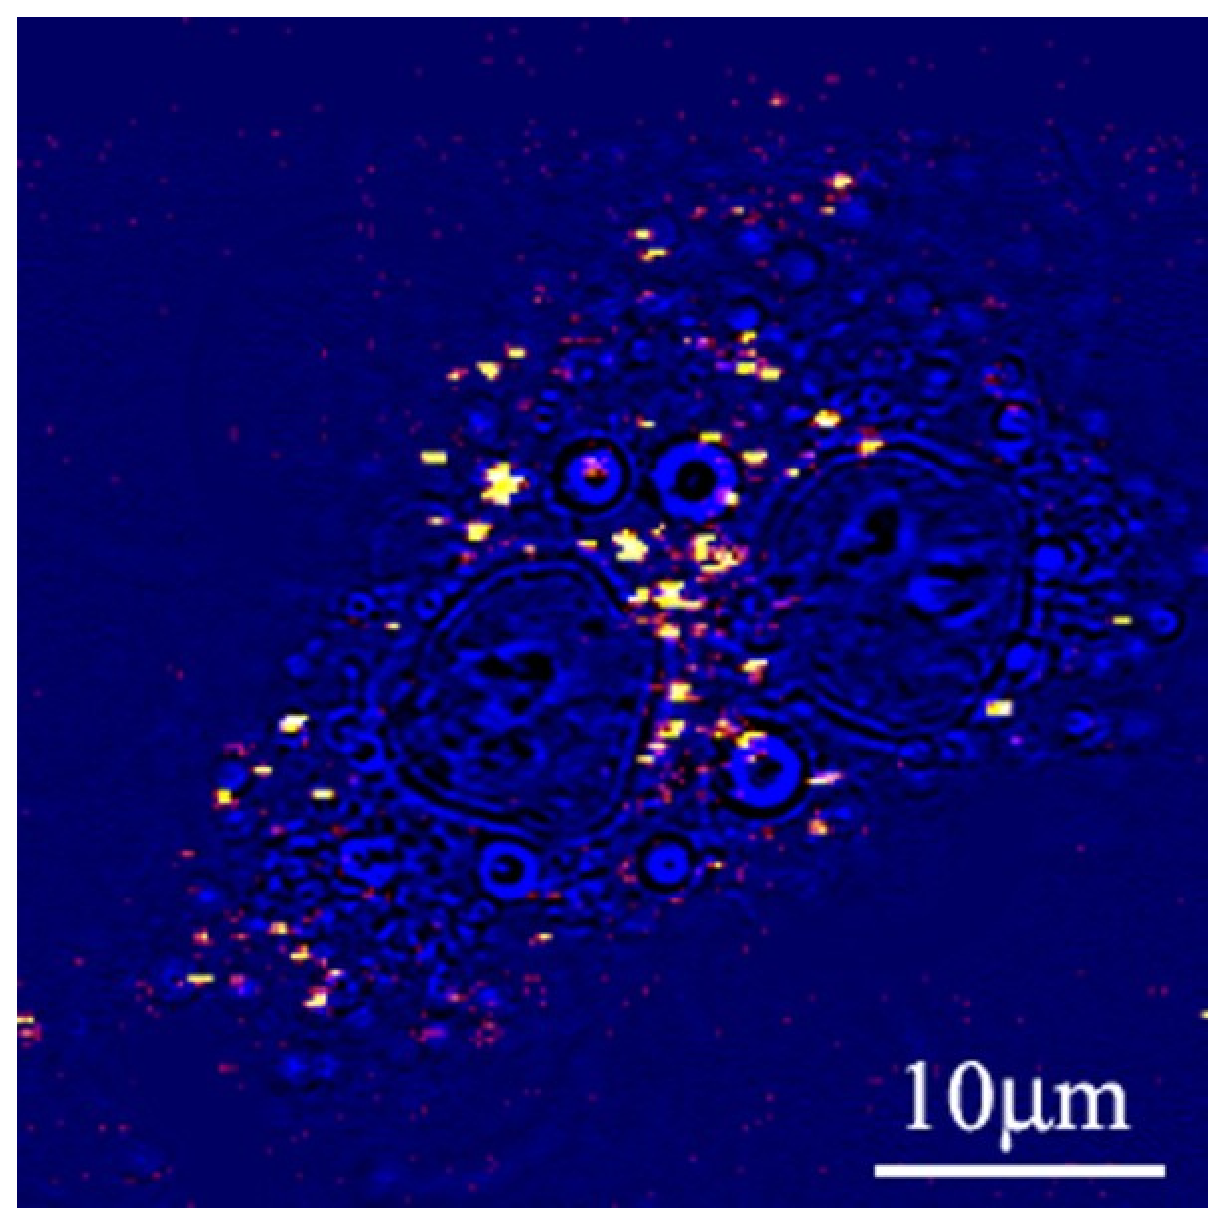
\includegraphics[width=7cm]{opexfig1}
\caption{Sample caption (Ref. \cite{Oron03}, Fig. 2).}
\end{figure}

\begin{equation}
H = \frac{1}{2m}(p_x^2 + p_y^2) + \frac{1}{2} M{\Omega}^2
     (x^2 + y^2) + \omega (x p_y - y p_x).
\end{equation}
\end{verbatim}

\section{Conclusion}
After proofreading the manuscript, compress your .TEX manuscript file and all figures (which should be in EPS format, or PDF format if you are using PDF-\LaTeX) in a ZIP, TAR or TAR-GZIP package. Prism, OSA’s article tracking system, will process in \LaTeX mode by default but will use PDF-\LaTeX if PDF figure files are detected. Note: TAR or TAR-GZIP is no longer required. All files must be referenced at the root level (e.g., file \texttt{figure-1.eps}, not \texttt{/myfigs/figure-1.eps}). If there is video or other multimedia, the associated files should be uploaded separately.

\end{document}
